\chapter{Taylor-Green vortex decay using Pair-interaction CA}

Taylor-Green vortex decay is standard benchmark problem used for evaluation of accuracy of CFD methods. We shall see how deterministic and non-deterministic PI fare on this problem.

The lattice was set-up with periodic boundary conditions, and with initial velocity field
\begin{align} \label{tginit}
\begin{split}
v_x &= \sin(\frac{2\pi}{I} \, x)\, \cos(\frac{2\pi}{I} \, y)\, \cos(\frac{2\pi}{I} \, z), \\
v_y &= -\cos(\frac{2\pi}{I} \, x)\, \sin(\frac{2\pi}{I} \, y)\, \cos(\frac{2\pi}{I} \, z), \\
v_z &= 0.
\end{split}
\end{align}
We can see that the above setup obeys the continuity equation
\begin{align*}
\nabla \times \bm{v} = 0.
\end{align*}

Functions below implements the Taylor-Green vortex with the initial conditions \ref{tginit}.
\begin{lstlisting}
//sets macroscopic velocity (vx,vy,vz) at (i,j,k)
void set_speed(Node***a, int i, int j, int k, int dx, int dy, int dz, double vx, double vy, double vz)
{
	double n = 0;
	int mx = 0;
	int my = 0;
	int mz = 0;

	unsigned char sx = vx >= 0 ? dirX : mirX;
	unsigned char sy = vy >= 0 ? dirY : mirY;
	unsigned char sz = vz >= 0 ? dirZ : mirZ;

	double absx = vx >= 0 ? vx : -vx;
	double absy = vy >= 0 ? vy : -vy;
	double absz = vz >= 0 ? vz : -vz;

	for (int x = i; x < i + dx; x += 2)
	{
		for (int y = j; y < j + dy; y += 2)
		{
			for (int z = k; z < k + dz; z += 2)
			{
				n += 1;
				if (mx / n < absx)
				{
					++mx;
					a[x][y][z].m |= sx;
					a[x][y][z].p[0] |= sx;
				}
				if (my / n < absy)
				{
					++my;
					a[x][y][z].m |= sy;
					a[x][y][z].p[1] |= sy;
				}
				if (mz / n < absz)
				{
					++mz;
					a[x][y][z].m |= sz;
					a[x][y][z].p[2] |= sz;
				}
			}
		}
	}
}

// sets initial conditions for taylor-green vortex
void taylor_green_vortex(Node***a, int I, int J, int K, int X, int Y, int Z, int dx, int dy, int dz)
{
	double ampl = 0.5;
	double kx = 2 * PI / I;
	double ky = 2 * PI / J;
	double kz = 2 * PI / K;

	double ax = 1 * ampl;
	double ay = -1 * ampl;
	double az = 0;

	double vx, vy, vz;

	for (int i = 0; i < I; ++i)
		for (int j = 0; j < J; ++j)
			for (int k = 0; k < K; ++k)
			{
				vx = ax * sin(kx * i) * cos(ky * j) * cos(kz * k);
				vy = ay * cos(kx * i) * sin(ky * j) * cos(kz * k);
				vz = 0;
				
				set_speed(a, i*dx, j*dy, k*dz, dx, dy, dz, vx, vy, vz);
			}
}
\end{lstlisting}

\section{Simulation of the vortex decay by deterministic and non-deterministic PI}

\begin{figure}[H]
 \centering 
 \includegraphics[width=0.9\textwidth]{../new_tgv/velocity_0}
 \label{transitions}
 \caption{Time 0 -- deterministic PI}
\end{figure}
\begin{figure}[H]
 \centering 
 \includegraphics[width=0.9\textwidth]{../new_tgv/velocity_4}
 \label{transitions}
 \caption{Time 4 -- deterministic PI}
\end{figure}

\begin{figure}[H]
 \centering 
 \includegraphics[width=0.9\textwidth]{../new_tgv/velocity_8}
 \label{transitions}
 \caption{Time 8 -- deterministic PI}
\end{figure}

\begin{figure}[H]
 \centering 
 \includegraphics[width=0.9\textwidth]{../new_tgv/velocity_12}
 \label{transitions}
 \caption{Time 12 -- deterministic PI}
\end{figure}


\begin{figure}[H]
 \centering 
 \includegraphics[width=0.9\textwidth]{../new_tgv/velocity_16}
 \label{transitions}
 \caption{Time 16 -- deterministic PI}
\end{figure}

\begin{figure}[H]
 \centering 
 \includegraphics[width=0.9\textwidth]{../new_tgv/velocity_20}
 \label{transitions}
 \caption{Time 20 -- deterministic PI}
\end{figure}


\begin{figure}[H]
 \centering 
 \includegraphics[width=0.9\textwidth]{../new_tgv/velocity_28}
 \label{transitions}
 \caption{Time 28 -- deterministic PI}
\end{figure}


\begin{figure}[H]
 \centering 
 \includegraphics[width=0.9\textwidth]{../new_tgv/velocity_108}
 \label{transitions}
 \caption{Time 108 -- deterministic PI}
\end{figure}


\begin{figure}[H]
 \centering 
 \includegraphics[width=0.9\textwidth]{../newest_taynon/velocity_0}
 \label{transitions}
 \caption{Time 0 -- NON-deterministic PI}
\end{figure}
\begin{figure}[H]
 \centering 
 \includegraphics[width=0.9\textwidth]{../newest_taynon/velocity_4}
 \label{transitions}
 \caption{Time 4 -- NON-deterministic PI}
\end{figure}

\begin{figure}[H]
 \centering 
 \includegraphics[width=0.9\textwidth]{../newest_taynon/velocity_8}
 \label{transitions}
 \caption{Time 8 -- NON-deterministic PI}
\end{figure}

\begin{figure}[H]
 \centering 
 \includegraphics[width=0.9\textwidth]{../newest_taynon/velocity_12}
 \label{transitions}
 \caption{Time 12 -- NON-deterministic PI}
\end{figure}


\begin{figure}[H]
 \centering 
 \includegraphics[width=0.9\textwidth]{../newest_taynon/velocity_16}
 \label{transitions}
 \caption{Time 16 -- NON-deterministic PI}
\end{figure}

\begin{figure}[H]
 \centering 
 \includegraphics[width=0.9\textwidth]{../newest_taynon/velocity_20}
 \label{transitions}
 \caption{Time 20 -- NON-deterministic PI}
\end{figure}


\begin{figure}[H]
 \centering 
 \includegraphics[width=0.9\textwidth]{../newest_taynon/velocity_28}
 \label{transitions}
 \caption{Time 28 -- NON-deterministic PI}
\end{figure}


\begin{figure}[H]
 \centering 
 \includegraphics[width=0.9\textwidth]{../newest_taynon/velocity_108}
 \label{transitions}
 \caption{Time 108 -- NON-deterministic PI}
\end{figure}

\section{Kinetic energy}
As the diagnostic quantity of our model, we computed mean kinetic energy 
\begin{align*}
E_k = \int_V \frac{1}{2}\rho u^2 \dd V.	
\end{align*}
and followed its time evolution.
Our results can be compared with reference solution computed by nodal Discontinuous Galerkin and Spectral difference methods presented in \cite{tgvref}.

\begin{figure}[H]
 \centering 
 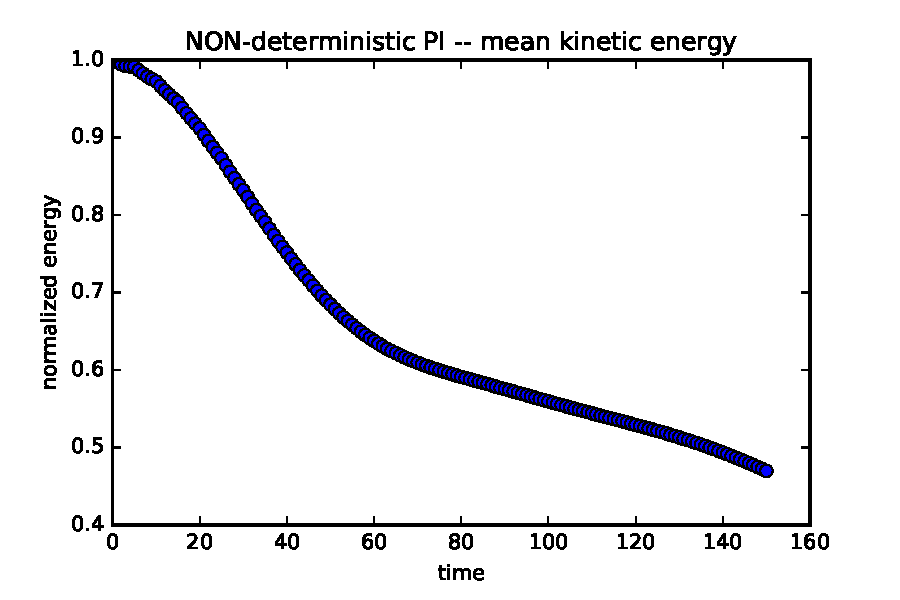
\includegraphics[width=1\textwidth]{./img/tgv_none}
\end{figure}

\begin{figure}[H]
 \centering 
 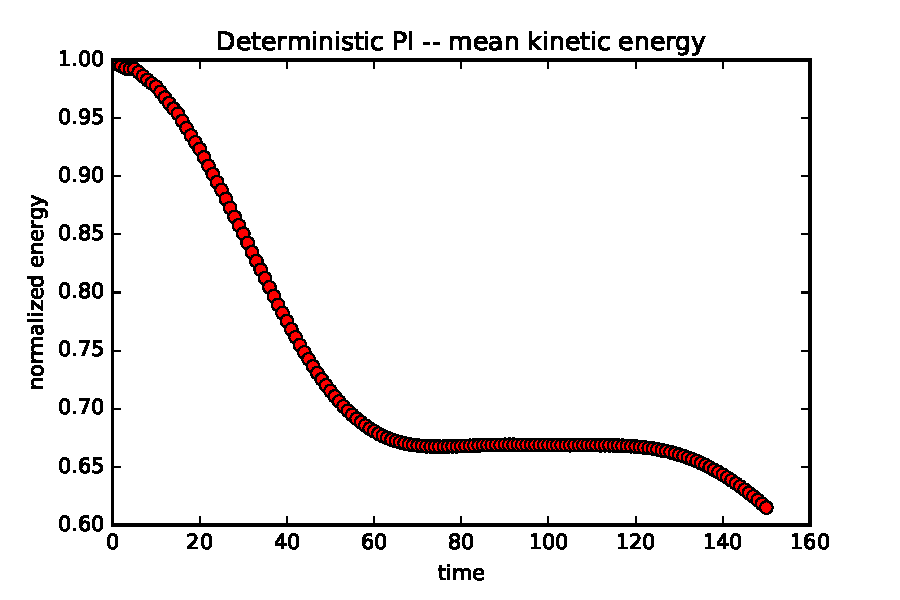
\includegraphics[width=1\textwidth]{./img/tgv_dete}
\end{figure}

In non-deterministic model, kinetic energy descends faster and more consistently, which agrees with our hypotheses that non-deterministic collision changes free paths of the particles more frequently.

\section{Computation speed and scaling}











